

%%%%%%%%%%%%%%%%%%%%%%%%%%%%%%%%%%%55%%
\begin{frame} [plain]
    \frametitle{}
    \Background[1] 
    \begin{center}
    {\huge 第2讲:量子逻辑门}
    \end{center}  
    \addtocounter{framenumber}{-1}   
\end{frame}
%%%%%%%%%%%%%%%%%%%%%%%%%%%%%%%%%%

\section{1.逻辑门的可逆性}

\begin{frame} 
    \frametitle{经典加法器}
    \begin{tcolorbox2}{信息学基本原理}
    所有类型的计算都是加法,二进制加法是逻辑运算,逻辑门是实现各种逻辑运算的基础性元件。
    \end{tcolorbox2}
    \例[1. 设计一个加法器,实现两整数之间的求和]{}
    \解~对于小于$2^n$的正整数$M,N$可表示为:
    \[M=\sum_{i=0} ^{n-1} a_i 2^i,\qquad N=\sum_{i=0} ^{n-1} b_i 2^i\]
\end{frame} 

\begin{frame}    
    \begin{table}
        \caption{加法器真值表,其中 $s_i, c_{i+1}$分别是求和位和进位}
        \begin{tabular}{@{} llll @{}}
          %\toprule
          $a_i$ & $b_i$ & $s_i$ & $c_{i+1}$\\
          \midrule
          0 & 0 & 0 & 0 \\
          0 & 1 & 1 & 0\\
          1 & 0 & 1 & 0\\
          1 & 1 & 0 & 1\\
          \bottomrule
        \end{tabular}
      \end{table}
    \begin{itemize}
        \IItem $a_i$, $b_i$ 不同时, $s_i$置“1”,否则置“0” : 逻辑“异或” XOR  $\qquad s_i=a_i\oplus b_i $
        \IItem $a_i$, $b_i$ 都是1时, $c_{i+1}$置“1”,否则置“0”:   逻辑“与” AND  $\quad c_{i+1}=a_i \wedge b_i $
    \end{itemize}
\end{frame} 

\begin{frame} 
    \frametitle{}
\centering
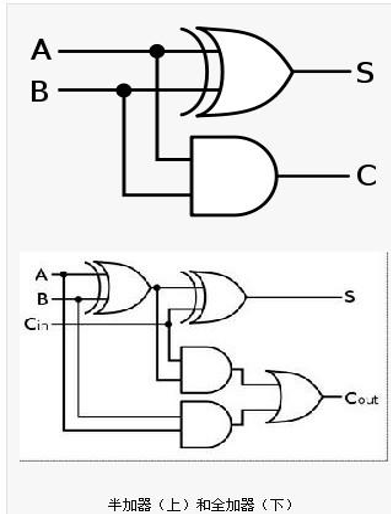
\includegraphics[width=0.45\textwidth]{figs/10.png}
\end{frame} 

\begin{frame} {可逆性}
    考察发现:经典 XOR 门和 AND 门都是不可逆的!\\
    不可逆过程有深刻的物理内含:
    \begin{itemize}
        \IItem 不可逆过程熵增加 $S=k_B\ln\Omega$
        \IItem 不可逆过程信息丢失 $\Delta S=k_B\ln2 $
        \IItem 不可逆过程消耗能量
        \IItem 不可逆过程不是幺正变换
    \end{itemize}
    当前通用的图灵机都是不可逆的! \\ \vspace{0.8em}
    {\Bullet}~~量子计算机通过酉操作(幺正变换)来实现信息处理,要求所有的逻辑门都是可逆的!\\
    
\end{frame}  

\begin{frame} 
    \begin{tcolorbox2}{Bennett 证明}
    所有不可逆的计算机都可以改造为可逆计算机
    \end{tcolorbox2}
    \例[2. 试把不可逆的异或门,改造为可逆的异或门]{}
    \解~改造方法如图 \\
    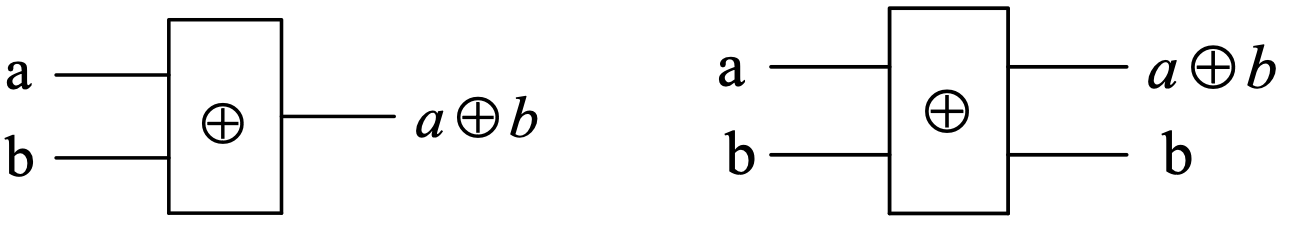
\includegraphics[width=0.7\textwidth]{figs/11.png}
    
    可逆源于所有信息被保留,信息的擦除消耗能量增加熵,导致不可逆。
\end{frame} 



\begin{frame}{}
        \frametitle{麦克斯韦妖佯谬-1871}
        绝热容器分成两格,中间是由“妖”控制的一扇“门”,分子作无规则热运动时会向门上撞击,“门”可以选择性的将速度较快的分子放入一格,
        较慢的分子放入另一格. 这样,体系的熵在减少!\\
       \begin{center}
        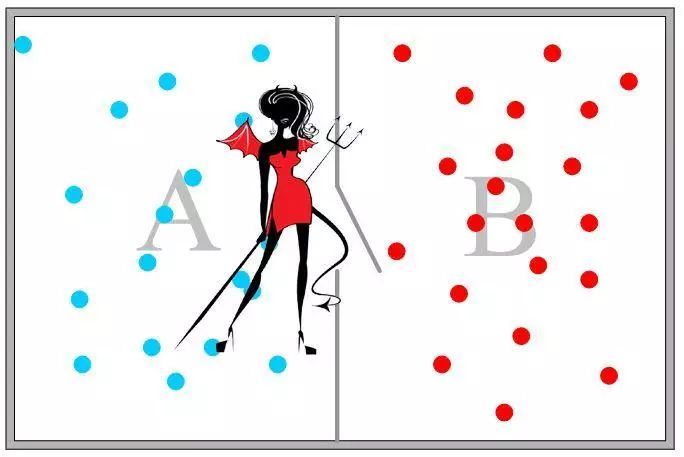
\includegraphics[width=0.42\textwidth]{figs/12.png}     
       \end{center}   
       1981年,Bennett证明“妖”必须去除前面分子的信息,这消耗能量并导致$k_B\ln2$的熵增。 
\end{frame} 

\begin{frame}
    基本结论:\\
   \begin{itemize}
       \IItem 微观过程是可逆的
       \IItem 微观过程服从量子力学原理
       \IItem 演化过程是幺正的
       \IItem 基于幺正变设计的量子逻辑门是可逆的
       \IItem 如果有一套普适的量子逻辑门,发展量子计算机是可行的
   \end{itemize} 
\end{frame} 

\section{2.单量子比特逻辑门}

\begin{frame}
    \frametitle{单量子比特逻辑门}   
    {\Bullet} 分析:单量子比特波函数
\[\rs{\psi} =\alpha\rs{0}+\beta\rs{1}, \qquad (|\alpha|^2+|\beta|^2=1)\]
矩阵:
 \[ \rs{\psi}=\begin{bmatrix}
    \alpha \\
    \beta
 \end{bmatrix}\]
 因此,\\
 (1)单比特逻辑门是操作$C^2$空间的$2\times 2$的矩阵,\\
 (2)单比特逻辑门必须是幺正(酉)矩阵(可逆性要求)
\end{frame} 

\begin{frame} 
    \frametitle{量子非门(X-Gate)-比特反转门} 
    经典非门: $0\to 1, \qquad 1 \to 0$ \\
    量子非门: $\alpha\rs{0}+\beta\rs{1} \quad \to \quad\alpha\rs{1}+\beta\rs{0}$ \\ \vspace{1em}

    \例[2. 试证明$\sigma_x$矩阵就是单比特量子非门]
    {~~\\
    \[X \equiv \sigma_x=\XGate = \rl{0}{1}+\rl{1}{0}\]} 
    \证~(1)量子非,对于$\rs{\psi} =\alpha\rs{0}+\beta\rs{1}$,有
    \[X \rs{\psi} = X \Qbit{\alpha}{\beta}=\XGate\Qbit{\alpha}{\beta} =\Qbit{\beta}{\alpha}=\beta\rs{0}+\alpha\rs{1}=\alpha\rs{1}+\beta\rs{0}
    \]
\end{frame} 

\begin{frame}     
    (2)幺正性
    \[X^\dagger =(X_{ij} ^*)^T=\XGate\]
    \[X^\dagger X = XX^\dagger =\XGate \XGate=I\]
    证毕!\\ \vspace{1em}
    {\Bullet} 很明显,这是比特反转
    \[ X\rs{0}= \rs{1},\qquad X\rs{1}= \rs{0}
    \]
\end{frame}

\begin{frame}{}
    比特反转的物理图像
    \begin{center}
        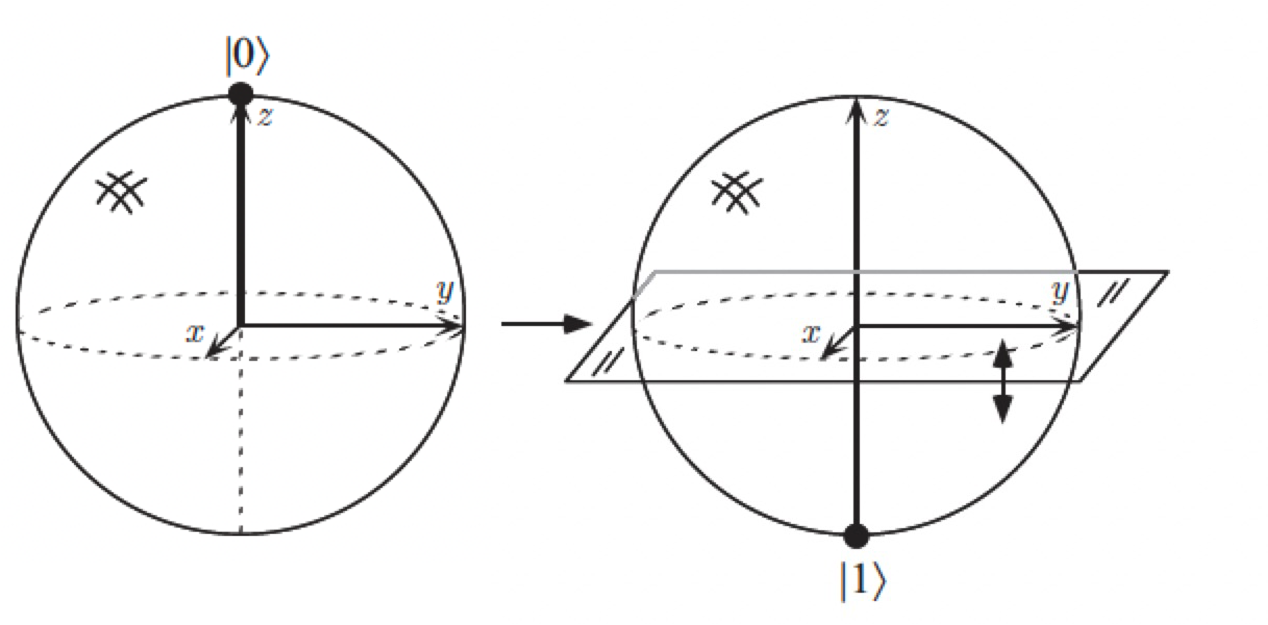
\includegraphics[width=0.8\textwidth]{figs/13.png}     
    \end{center}  
\end{frame}

\begin{frame}{基矢变换门(H-Gate)}
    基矢变换: $\rs{0} \to \rs{+} =\Pstate, \qquad \rs{1} \to \rs{-} =\Mstate $ \\
    物理图像:把z方向的基矢变换成x方向的基矢
    \begin{center}
        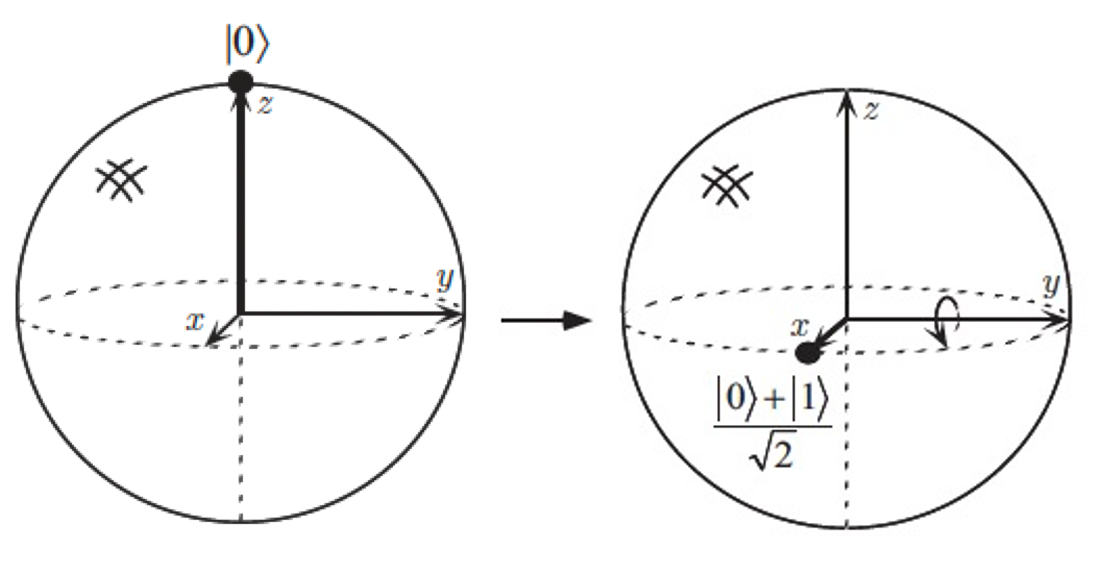
\includegraphics[width=0.7\textwidth]{figs/14.png}     
    \end{center} 
\end{frame}

\begin{frame}
    \frametitle{}
    \例[4. 试证明如下矩阵就是基矢变换门]
    {~~\\
    \[H \equiv \frac{1}{\sqrt{2}}(X+Z) =\HGate \]} 
    \证~(1)基矢变换
    \[H \rs{0}= \HGate\Qbit{1}{0}=\frac{1}{\sqrt{2}}\Qbit{1}{1} = \frac{1}{\sqrt{2}}\Qbit{1}{0} +\frac{1}{\sqrt{2}}\Qbit{0}{1} =\frac{\rs{0}+\rs{1}}{\sqrt{2}} =\rs{+}\]
    \[\text{同理}\qquad H \rs{1}=\frac{\rs{0}-\rs{1}}{\sqrt{2}} =\rs{-}\]
\end{frame}

\begin{frame}{}
    (2)幺正性
    \[H^\dagger H = HH^\dagger=I\]
    证毕! \\ \vspace{0.6em}
    \[H \rs{0}=\frac{\rs{0}+\rs{1}}{\sqrt{2}}\]
    \[H \rs{1}=\frac{\rs{0}-\rs{1}}{\sqrt{2}}\]
    {\Bullet} 统一表示为:(x,z 分别取0或1)\\
    \[H \rs{x}=\frac{\sum_z(-1)^{xz}\rs{z}}{\sqrt{2}}\]
\end{frame}

\begin{frame}
    \frametitle{}
    {\Bullet} 很明显~H~是自共轭矩阵,有: \[H^\dagger =H \to H^2=I\]
    \例[5. 试证明H可以完成反向变换]
    {~~\\
    \[H \rs{+}= \rs{0}, \qquad H \rs{-}= \rs{1}  \]} 
    \证~ \[H\rs{0}=\rs{+}, \qquad H \rs{0}= \rs{-} \]
    \[HH\rs{0}=H\rs{+} , \qquad H H\rs{0}= H\rs{-}\]
    \[\rs{0}=H\rs{+} , \qquad \rs{0}= H\rs{-}\]
    证毕!
\end{frame}

\begin{frame}
    \frametitle{相位反转门(Z-Gate)} 
    相位反转: $\alpha\rs{0}+\beta\rs{1} \quad \to \quad\alpha\rs{0}-\beta\rs{1}$ \\ \vspace{0.6em}
    \例[3. 试证明$\sigma_z$矩阵就是相位反转门]
    {~~\\
    \[Z \equiv \sigma_z =\ZGate =-i\rl{0}{1}+i\rl{1}{0}\]} 
    \证~(1)相位反转
    \[Z \Qbit{\alpha}{\beta}=\ZGate\Qbit{\alpha}{\beta} =\Qbit{\alpha}{-\beta}\]
    (2)幺正性
    \[Z^\dagger Z = ZZ^\dagger=I\]
    证毕!~~ {\Bullet} 很明显~~$ Z\rs{0}=\rs{0},\quad Z\rs{1}=-\rs{1}= e^{i\pi}\rs{1}$
\end{frame}

\begin{frame}
    \frametitle{旋转门} 
    既然态矢都在 Block球面,相位反转(Z-Gate)就是绕Z轴旋转180度($\pi$)(为什么?)\\
    {\Bullet}绕Z轴旋转90度($\dfrac{\pi}{2}$)的门是S-Gate.\\
    \[Z\rs{1}= e^{i\pi}\rs{1}\]
    \[S\rs{1}= e^{i\pi/2}\rs{1}\]
    解得:
    \[S \equiv \SGate = {\begin{bmatrix}
        1 & 0 \\
        0 & e^{\frac{i\pi}{2}}
     \end{bmatrix}}\]
    由于$i=\sqrt{-1}$,也称S-Gate 为$\sqrt{Z}$-Gate 
\end{frame}
    
\begin{frame}
    \frametitle{}
    {\Bullet}绕Z轴旋转45度的门为T-Gate,也称 $\pi/8$-Gate
    \[T \equiv {\begin{bmatrix}
        1 & 0 \\
        0 & e^{\frac{i\pi}{4}}
     \end{bmatrix}} = e^{\frac{i\pi}{8}} {\begin{bmatrix}
        e^{\frac{-i\pi}{8}} & 0 \\
        0 & e^{\frac{i\pi}{8}}
     \end{bmatrix}}\]
    {\Bullet}绕Z轴旋转任意角度($\varphi$)的门为旋转门$R_z(\varphi)$-Gate
    \[R_z(\varphi) \equiv  \RGate \]
\end{frame}

\begin{frame}
    \frametitle{}
    {\Bullet}不失一般性,存在各方向的旋转门
    \[R_z(\theta) \equiv e^{-i\theta Z/2}\]
    \[R_y(\theta) \equiv e^{-i\theta Y/2}\]
    \[R_x(\theta) \equiv e^{-i\theta X/2}\]
    \[R_{\hat{n}}(\theta) \equiv e^{-i\theta \hat{n}\cdot \sigma/2}\]
\end{frame}

\begin{frame}
    \frametitle{}
    小结:常用单比特量子门\\
    \begin{center}
        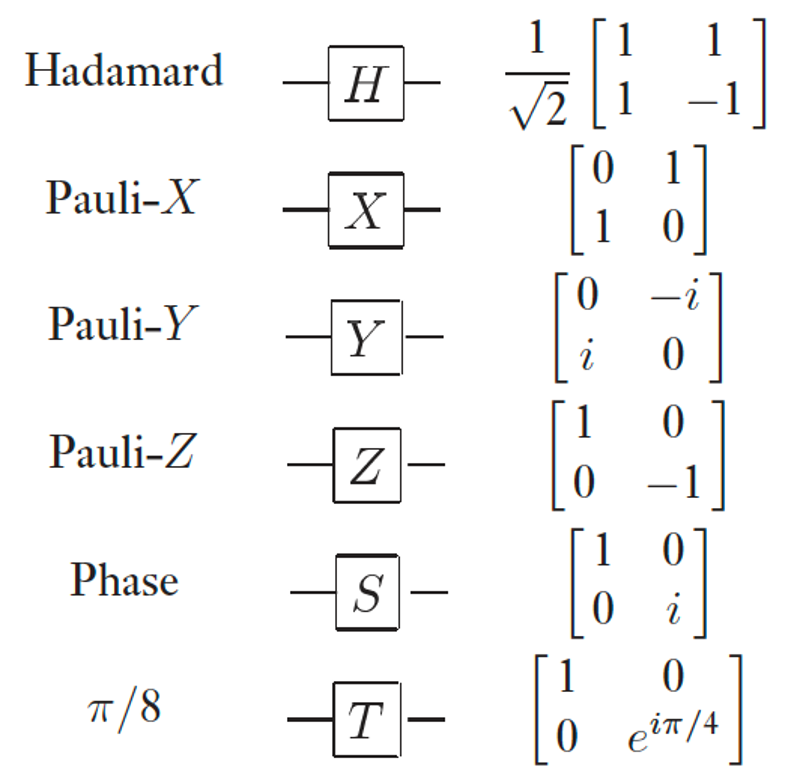
\includegraphics[width=0.5\textwidth]{figs/15.png}     
    \end{center} 
    它们都是幺正($U$)门
\end{frame}

\section{3.多量子比特逻辑门}
\begin{frame}
    \frametitle{多量子比特逻辑门}
    1.控制非门 (Controlled-Not-Gate)\\
    \[ C-NOT\equiv {\begin{bmatrix}
        1 & 0 & 0 & 0\\
        0 & 1 & 0 & 0\\ 
        0 & 0 & 0 & 1\\ 
        0 & 0 & 1 & 0
     \end{bmatrix}}
    \]
    \begin{center}
        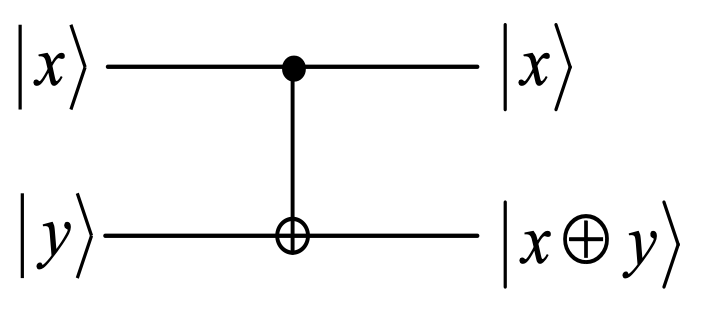
\includegraphics[width=0.35\textwidth]{figs/16.png}     
    \end{center} 
\end{frame}

\begin{frame}
    \frametitle{}
    \[\text{输入} \qquad \qquad \qquad \text{输出}\] 
    \[\rs{x}\rs{y}\qquad \qquad \rs{x}\rs{x \oplus y}\]
    \[\rs{00} \qquad \qquad \qquad \rs{00} \]
    \[\rs{01} \qquad \qquad \qquad \rs{01} \]
    \[\rs{10} \qquad \qquad \qquad \rs{11} \]
    \[\rs{11} \qquad \qquad \qquad \rs{10} \]
    {\Bullet}控制位(x)置位时,对目标位(y)做非操作
\end{frame}

\begin{frame}
    \frametitle{}
    2. 交换门 (Switch-Gate)
    \begin{center}
        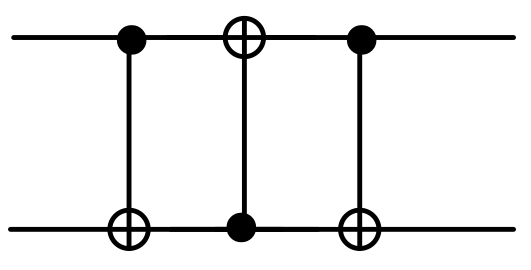
\includegraphics[width=0.32\textwidth]{figs/17.png}     
    \end{center} 
    \[\text{输入} \rs{a,b} \qquad \to \qquad \text{输出} \rs{b,a} \] 
    \证 
    \[\rs{a}\rs{b} \to \rs{a}\rs{a \oplus b }\]
    \[\rs{a}\rs{a \oplus b } \to \rs{a\oplus(a \oplus b )}\rs{a \oplus b } = \rs{b}\rs{a \oplus b} \]
    \[\rs{b}\rs{a \oplus b} \to \rs{b}\rs{b \oplus (a \oplus b} = \rs{b}\rs{a}\]
    证毕!
\end{frame}

\begin{frame}
    \frametitle{}
    3.  控制$U$门 ($U_0: I, U_1:X, U_2:Y,U_3:Z,\cdots$)
    \begin{center}
        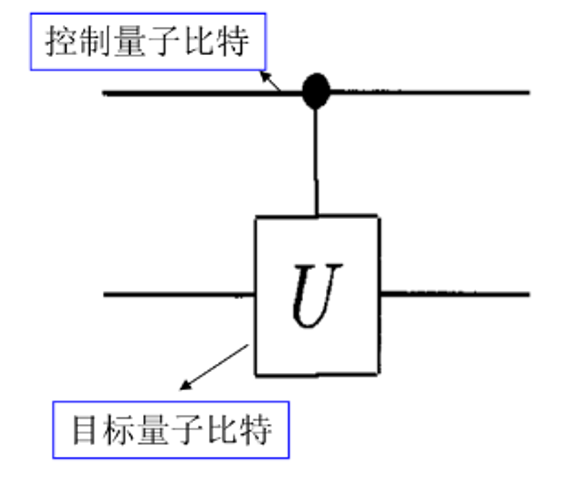
\includegraphics[width=0.35\textwidth]{figs/18.png}     
    \end{center} 
   功能:$U$是单量子比特的任意酉算子。如果控制位置位,则U作用到目标位上,否则目标位不变。
    \[\rs{c}\rs{t} \to \rs{c}U^c\rs{t}\]
    显然,当U=X时,就是控制非门(CNOT)
\end{frame}

\begin{frame}
    \frametitle{}
    {\Bullet}通过设计一系列的控制$U$门,我们可以控制系统的初态向目标态的演化!\\ \vspace{0.8em}
    依据:量子力学的演化假设,薛定谔方程与酉变换等价,有:
    {\Large \[\rs{\text{末态}}=\prod_{i} U_i\rs{\text{初态}} \]}
\end{frame}

\begin{frame}
    \frametitle{}
    4.  双控制位的控制$U$门 ($C^2(U)$) 
    \begin{center}
        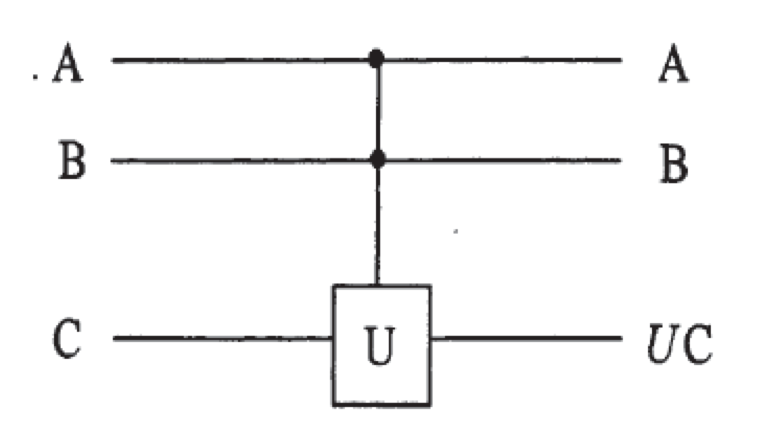
\includegraphics[width=0.35\textwidth]{figs/19.png}     
    \end{center} 
   功能:只有当两个控制位都置位时,U才作用到目标位上,否则目标位不变。
    显然,当U=X时,就是控制非门(CNOT)
\end{frame}

\begin{frame}
    \frametitle{}
    例.  下面的Toffoli门,就是双控制位的控制非(X)门
    \begin{center}
        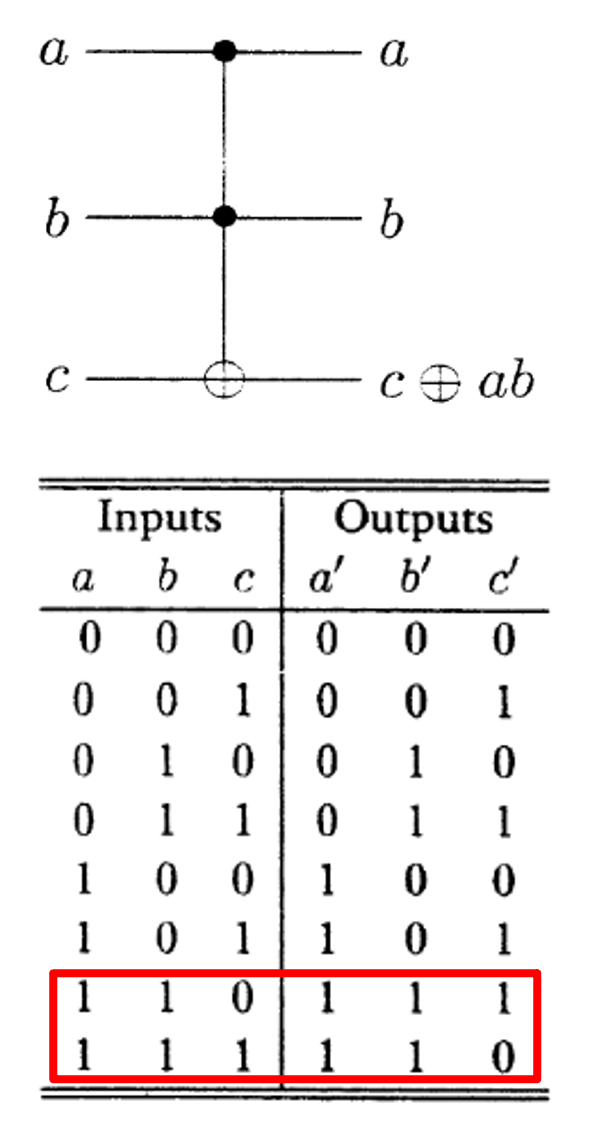
\includegraphics[width=0.30\textwidth]{figs/20.png}     
    \end{center} 
\end{frame}

\begin{frame}
    \frametitle{}
    \centering
    \tcbb[0.68]{深刻意义}
    {Toffoli门是可逆门,是实现普适计算的基础。可以证明:经典条件下一位两位可逆门不足以实现Toffoli门。而量子条件下由H,CNOT,S和 T门可以任意精度地近似任意酉操作。
    也就是说,只有在量子条件下,才可以实现普适的可逆计算!}
\end{frame}

\begin{frame}
    \frametitle{}
    \begin{center}
        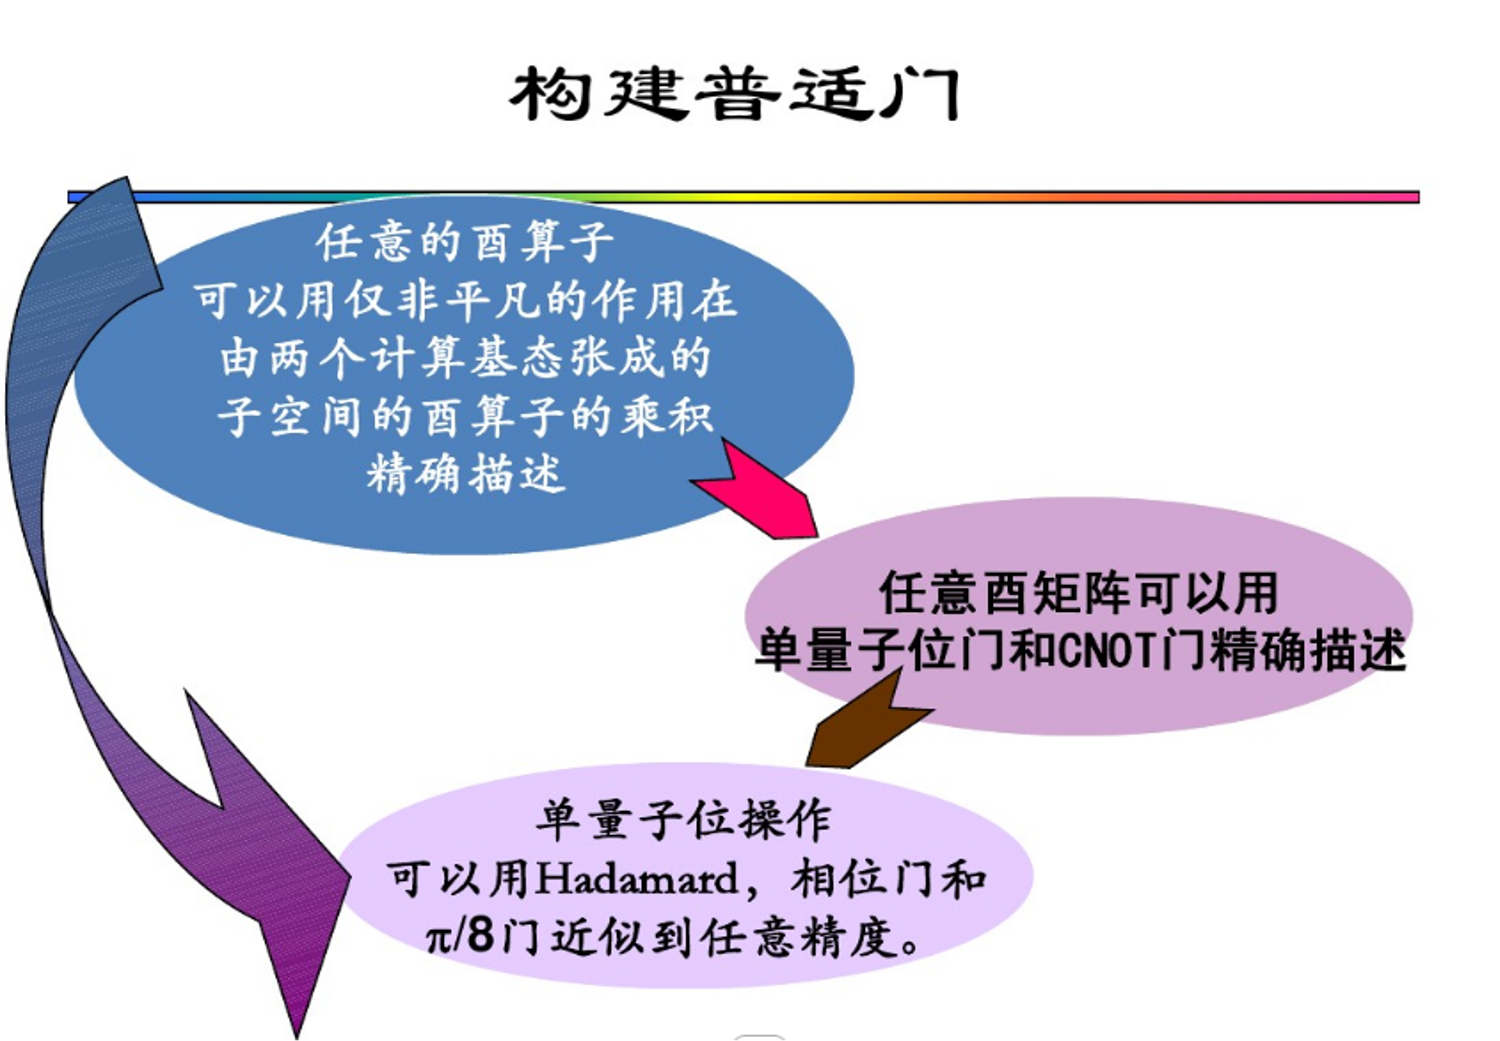
\includegraphics[width=0.85\textwidth]{figs/21.png}     
    \end{center} 
\end{frame}


\begin{frame}
    \frametitle{}
    \begin{tcolorbox3}[讨论专题]
    设光子偏振态与计算基矢态有如下关系:
    \begin{center}
        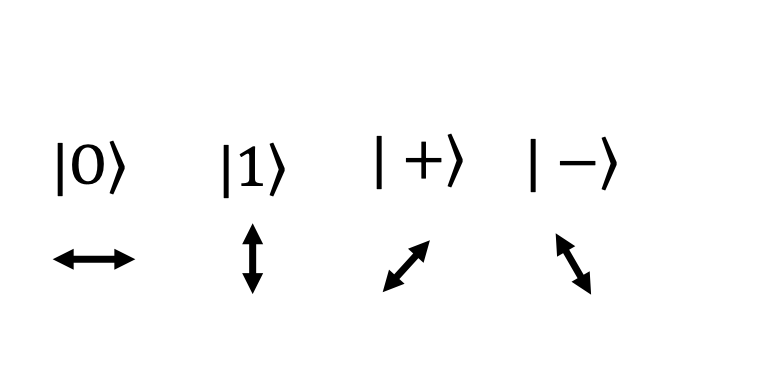
\includegraphics[width=0.35\textwidth]{figs/23.png}     
    \end{center}  
    试设计普适计算所必须的H,CNOT,S和 T门   
    \end{tcolorbox3}
\end{frame}

\begin{frame}
    \frametitle{}
    5.  多控制位多目标位的控制$U$门 ($C^n(U_k)$) 
    \begin{center}
        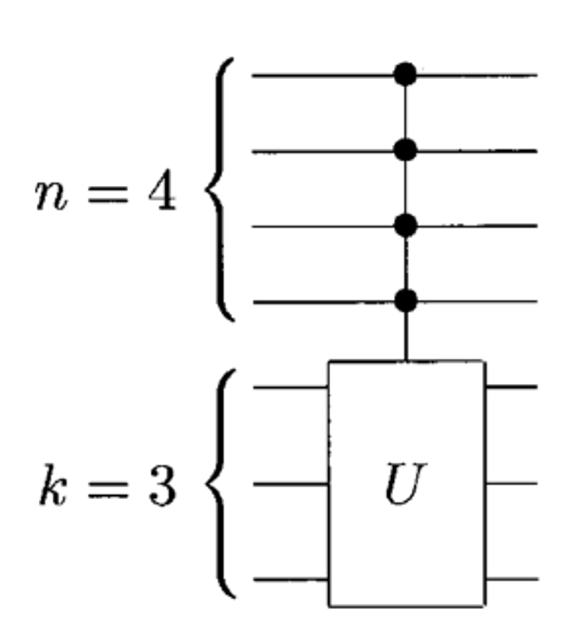
\includegraphics[width=0.31\textwidth]{figs/22.png}     
    \end{center} 
   功能:只有当所有控制位都置位时,U才作用到目标位上,否则目标位不变。
\end{frame}

\begin{frame}
    \frametitle{}
    6.  经典函数的量子门阵列实现
    \begin{center}
        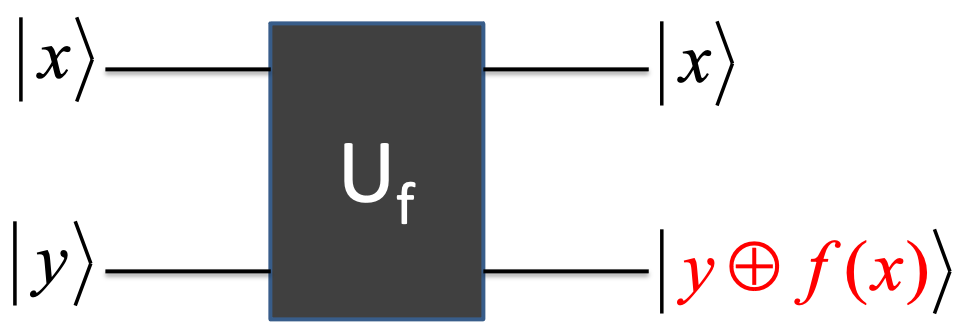
\includegraphics[width=0.38\textwidth]{figs/25.png}     
    \end{center} 
    \begin{itemize}
        \IItem 任意经典函数都可以转化成二进位形式下的一系列逻辑运算,这些逻辑运算由量子门阵列$U_f$实现
        \IItem 输入位$\rs{x}$,经$U_f$运算后,得到函数值$f(x)$
        \IItem $f(x)$要么是0要么是1,只有当$f(x)=1$时,才对目标位(y)做非操作,否则目标位不变。
    \end{itemize}
    \[U_f\rs{x,y}\qquad \to \qquad \rs{x,y\oplus f(x)}\]
\end{frame}

\begin{frame}
    \frametitle{作业}
    这是一个量子加法器
    \begin{center}
        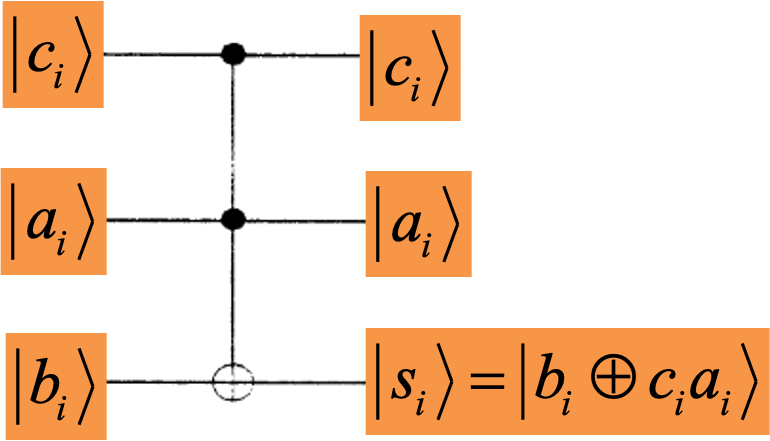
\includegraphics[width=0.38\textwidth]{figs/24.png}     
    \end{center} 
    \[\rs{a,b}\qquad \to \qquad \rs{a,a+b}\]
    试给出真值表
\end{frame}
